\chapter{Revisão Bibliográfica}

\section{Mercado de Veículos Elétricos}

\section{Estações de carregamento - EVSE}

O carregamento de veículos elétricos é realizado por meio de estações de carregamento (EVSE). O padrão IEC 62196 \cite{iec62196} tenta padronizar alguns dos conectores já usados no mercado, assim como os modos de operações de uma estação de carregamento.

\subsection{Padrões de Conectores}

\subsection{Modos de Operação}

\section{Protocolos de Comunicação - EVSE}

As estações de carregamento normalmente se comunicam com um servidor central, que pode gerenciar N estações. Para tal tarefa, é necessário um protocolo de comunicação. Embora não haja um padrão oficial, alguns protocolos já se sobressaem em questões de utilização pelo indústria.

\subsection{OCPP}

O OCPP - Open Charge Point Protocol - foi criado pela Open Charge Alliance e hoje está presente em 50 países e em mais de 10000 estações de carregamento. Na Europa, todas estações comercializadas precisam ser compatíveis com o OCCP.

O protocolo prevê um sistema central que recebe dados de N estações. Caso for necessário, o sistema central pode atuar sob tais estações com ações como reservar a estação, cancelar algum carregamento ou até desligar a estação. Caso a estação perca conectividade, o protocolo prevê que ela deve funcionar de modo autônomo, somente registrando alguns dados para envio posterior (início e finalização de carregamentos).

As requisições da versão 1.5 podem ser via SOAP ou WebSocket, enquanto a versão 1.6 já adiciona suporte a JSON.

\section{Protocolo MODBUS}

Em projetos industriais, é requisito que dispositivos diversos consigam comunicar-se entre si. Para tal, existem dezenas de protocolos que permitem a realização dessa tarefa, sendo o MODBUS um dos mais comuns \cite{modbusspec}. Sua implementação inicial era sob serial, porém hoje também é possível utilizar o stack TCP/IP e outras implementações menos comuns - UDP, PEMEX, Enron.

\subsection{Funcionamento}

O protocolo é baseado no modelo mestre-escravo, onde um dispositivo mestre requisita os dados dos dispositivos escravos. Essa analogia é muito semelhante ao modelo cliente-servidor, onde o cliente seria o mestre e o servidor o escravo.

\begin{figure}[H]
        \begin{center}
                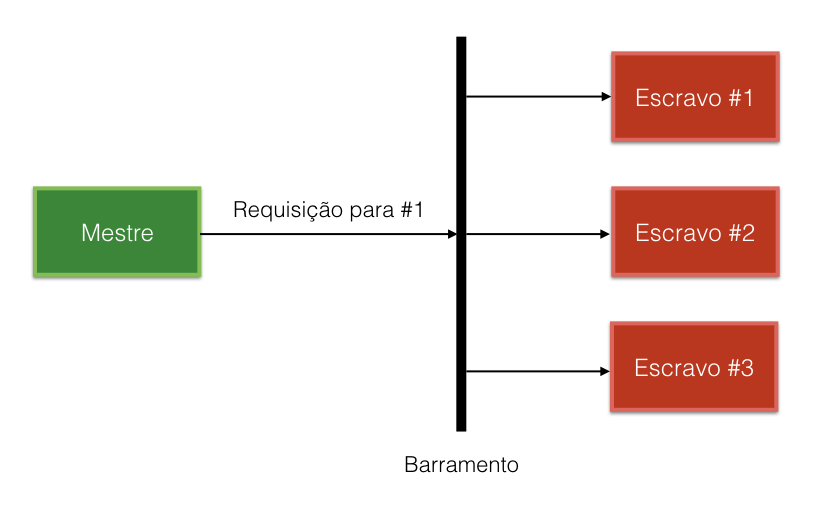
\includegraphics[width=\textwidth,natwidth=1024,natheight=768]{assets/images/modbus-req-1.png}
                \caption{Requisição MODBUS do mestre para o escravo}
                \label{fig:modbus-req-1}
        \end{center}
\end{figure}

Como uma rede pode ter N escravos, cada escravo possui um endereço atribuído. O mestre envia a requisição para o barramento e todos os escravos a recebem, porém somente o endereçado responderá. Há também a opção de se fazer um broadcast - endereço 0 - onde todos escravos recebem a requisição, porém nesse caso nenhum escravo deve responde-lá.

Vale notar que uma rede MODBUS-RTU há somente um mestre, enquanto em uma rede MODBUS-TCP é possível que cada mestre seja um escravo, e vice-versa.

\begin{figure}[H]
        \begin{center}
                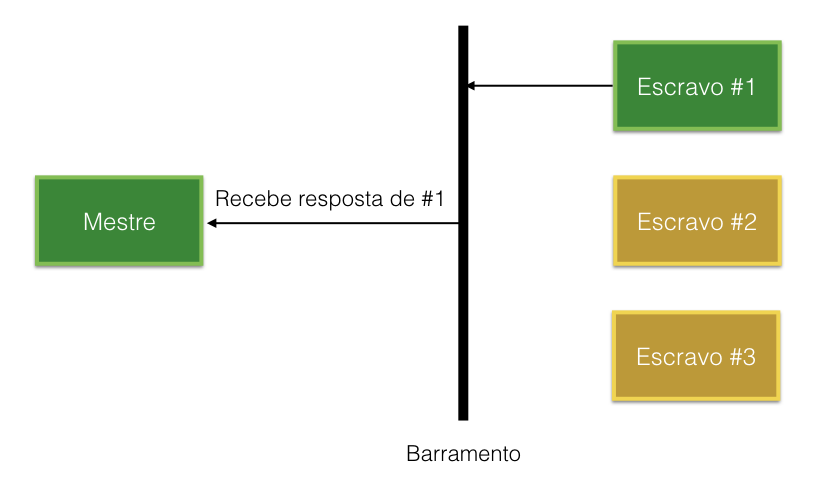
\includegraphics[width=\textwidth,natwidth=1024,natheight=768]{assets/images/modbus-req-2.png}
                \caption{Resposta MODBUS do escravo para o mestre}
                \label{fig:modbus-req-2}
        \end{center}
\end{figure}

\subsection{Mapa de Memória}

Toda requisição realizada pelo mestre endereçará um dado no mapa de memória do dispositivo escravo, sendo que tal mapa de memória normalmente é indicado por uma documentação. Os dados requisitados podem possuir quatro tipos distintos:

\begin{itemize}
  \item Input: dado binário que permite apenas leitura
  \item Coil: dado binário que permite leitura e escrita
  \item Input Register: registrador com 16 bits (inteiro) que permite apenas leitura
  \item Holding Register: registrador com 16 bits (inteiro) que permite leitura e escrita
\end{itemize}

Para a realização de operações nesse mapa de memória, o mestre necessita informar nas suas requisições um function code. Este indicará qual dado deseja-se requisitar e se será executada uma operação de leitura ou escrita. A tabela mostra os mais comuns, porém existem mais códigos, aos quais podem ser usados para diagnósticos e entre outras funções.

\begin{table}[]
\centering
\caption{Function codes / Operações do MODBUS}
\label{modbus-funccodes}
\begin{tabular}{@{}ll@{}}
\toprule
\textbf{Operação}              & \textbf{Function code} \\ \midrule
Leitura de Coils               & 1                      \\
Escrita em 1 Coils             & 5                      \\
Escrita em N Coils             & 15                     \\
Leitura de Inputs              & 2                      \\
Leitura de Input Registers     & 4                      \\
Leitura de Holding Registers   & 3                      \\
Escrita em 1 Holding Register  & 6                      \\
Escrita em N Holding Registers & 16                     \\ \bottomrule
\end{tabular}
\end{table}

\subsection{Envio de informações}

Cada implementação possui algumas diferenças, porém o meio que as informações são organizadas e enviadas é o mesmo. Na imagem a seguir, é possível observar que em ambas implementações é necessária a definição de um FCode (function code). Esse definirá se a requisição será de leitura ou escrita e que tipo de dado será requisitado. Logo após vem o campo Data, onde pode ser indicado o endereço inicial do mapa de memória, quantos registradores deseja-se requisitar e quais dados serão escritos (no caso de escrita).

\begin{figure}[H]
        \begin{center}
                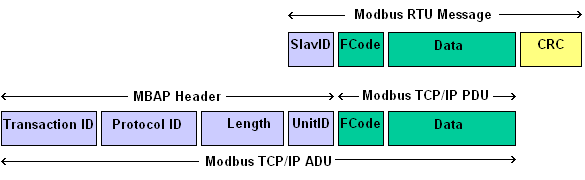
\includegraphics[width=\textwidth,natwidth=585,natheight=180]{assets/images/modbus-frame.png}
                \caption{Frame de Comunicação MODBUS}
                \label{fig:modbus-frame}
        \end{center}
\end{figure}

Como pode-se notar, somente no MODBUS-RTU há o SlavID (endereço), já que os dispositivos MODBUS-TCP são endereçados por seus IPs. O campo CRC é um dado que permite checar se o pacote obtido possui ou não algum erro. Como o protocolo TCP/IP já possui um meio para isso, tal campo não é incluído na requisição.

Esse formato de envio de informações é mantido tanto para requisição quanto para resposta, sendo que as respostas sempre possuíram o mesmo function code da requisição. Caso o function code diferir, provavelmente ocorreu um erro e este pode ser processado pelo mestre posteriormente.

\section{WSDL e SOAP}

O WSDL \cite{wsdlspec} permite descrever serviços web por meio de um arquivo XML. É possível definir os \textit{endpoints} - pontos de entrada para requisições - assim como o que devem retornar e o que devem receber como parâmetro. Isso permite que um serviço web seja desenvolvido por uma equipe que, posteriormente, exporta um WSDL do seu \textit{software}, descrevendo de maneira fácil quais são seus endpoints e facilitando a criação de clientes para o serviço.

Os arquivos WSDL definem suas interfaces em SOAP \cite{soapspec}, um protocolo que permite trocas de informações entre clientes e servidores de forma padronizada. Ele é baseado em XML e é montado em três partes:
\begin{itemize}
  \item Envolpe: identifica o que é a mensagem e como processá-la
  \item Cabeçalho: define informações extras sobre a mensagem
  \item Corpo: define o o procedimento a ser chamado e os dados de sua resposta
\end{itemize}

Como ele foi idealizado em XML, ele é facilmente processado por qualquer linguagem de programação, o que garante uma boa portabilidade.
